\documentclass[a4paper]{ctexart}

\usepackage[a4paper,hmargin={2.54cm,2.54cm},vmargin={3.175cm,3.175cm}]{geometry}
\usepackage{amsmath, amssymb}
\usepackage{amsthm}
\usepackage{graphicx}
\usepackage{physics}
\usepackage{xcolor}
\usepackage{caption}
\usepackage{subfig}
\usepackage{tikz}
\usepackage{float}
\usepackage{amsfonts}
\usepackage{svg}
\usepackage{verbatim}
\usepackage{quantikz}

\usepackage{cleveref}

\usepackage{algorithm}
\usepackage{algpseudocode}

\DeclareMathOperator{\fl}{\text{fl}}
\DeclareMathOperator{\Order}{\text{O}}
\DeclareMathOperator{\Real}{\mathbb R}
\newcommand{\pf}{\textbf{\color{pink}{proof:}}}

\newcommand{\bymn}[2]{$#1$-by-$#2$}
\newcommand{\ttmat}[4]{\begin{pmatrix}#1&#2\\#3&#4\end{pmatrix}}
\newcommand{\tmat}[2]{\begin{pmatrix}#1&#2\end{pmatrix}}
%\newcommand{\norm2}[1]{{\norm{#1}}_2}
\newcommand{\normf}[1]{{\norm{#1}}_F}

\begin{document}

\title{Chapter1}
\author{Guorui Zhu}
\maketitle

\section{}

\subsection{} 
Let $A$ be an orthogonal matrix. Show that
$\det(A) = \pm 1$. Show that if $B$ also is orthogonal and $\det(A) = -det(B)$, then
$A + B$ is singular.

\pf

\subsection{}
The rank of a matrix is the dimension of the
space spanned by its columns. Show that $A$ has rank one if and only if $A = ab^\top$
for some column vectors $a$ and $b$.

\pf

\subsection{}
Show that if a matrix is orthogonal and trian-
gular, then it is diagonal. What are its diagonal elements.

\pf

\subsection{}
A matrix is strictly upper triangular if it is
upper triangular with zero diagonal elements. Show that if $A$ is strictly upper
triangular and $n$-by-$n$, then $A^n = 0$.

\pf

\subsection{}
Let $\norm{\cdot}$ be a vector norm on $\mathbb R^m$ and assume
that $C \in \mathbb R^{m\times n}$. Show that if rank$(C) = n$, then $\norm{x}_C:=\norm{Cx}$ is a vector
norm.

\pf

\subsection{}
Show that if $0 \neq s \in \mathbb R^n$ and $E \in \mathbb R^{n\times n}$, then
\begin{equation*}
    \norm{E(I-\frac{ss^\top}{s^\top s})}^2_F = \norm{E}_F^2 - \frac{\norm{Es}_2^2}{s^\top s}.
\end{equation*}

\pf

\subsection{}
Verify that $\norm{xy^H}_F = \norm{xy^H}_2 = \norm{x}_2\norm{y}_2$ for
any $x, y \in \mathbb C^n$.

\pf

\subsection{}
One can identify the degree $d$ polynomials $p(x) = \sum_{i=0}^d a_i x^i$ with $\mathbb R^{d+1}$ via the vector of coefficients. 
Let $x$ be fixed. Let $S_x$ be
the set of polynomials with an infinite relative condition number with respect
to evaluating them at $x$ (i.e., they are zero at $x$). In a few words, describe $S_x$
geometrically as a subset of $\mathbb R^{d+1}$. Let $S_x(\kappa)$ be the set of polynomials whose
relative condition number is $\kappa$ or greater. Describe $S_x(\kappa)$ geometrically in a
few words. Describe how $S_x(\kappa)$ changes geometrically as $\kappa \to \infty$.

\pf

\subsection{}
Consider the figure below. 
It plots the function $y = \frac{\log (1 + x)}{x}$ computed in two different ways.
Mathematically, $y$ is a smooth function of $x$ near $x = 0$, equaling $1$ at $0$. But
if we compute $y$ using this formula, we get the plots in \cref{fig:1.9} on the left (shown in the
ranges $x \in [-1, 1]$ on the top left and $x \in [-10^{-15}, 10^{-15}]$ on the bottom left).
This formula is clearly unstable near $x = 0$. On the other hand, if we use the
algorithm
\begin{align*}
    &d=1+x\\
    &\text{if} \;d=1 \;\text{then}\\
    &\quad\quad y=1\\
    &\text{else}\\
    &\quad\quad y=\frac{\log(d)}{d-1}\\
    &\text{end if}
\end{align*}
we get the two plots on the right, which are correct near $x = 0$. Explain this
phenomenon, proving that the second algorithm must compute an accurate
answer in floating point arithmetic. Assume that the log function returns an
accurate answer for any argument. (This is true of any reasonable implemen-
tation of logarithm.) Assume IEEE floating point arithmetic if that makes
your argument easier. (Both algorithms can malfunction on a Cray machine.)
\begin{figure}[ht]
    \centering
    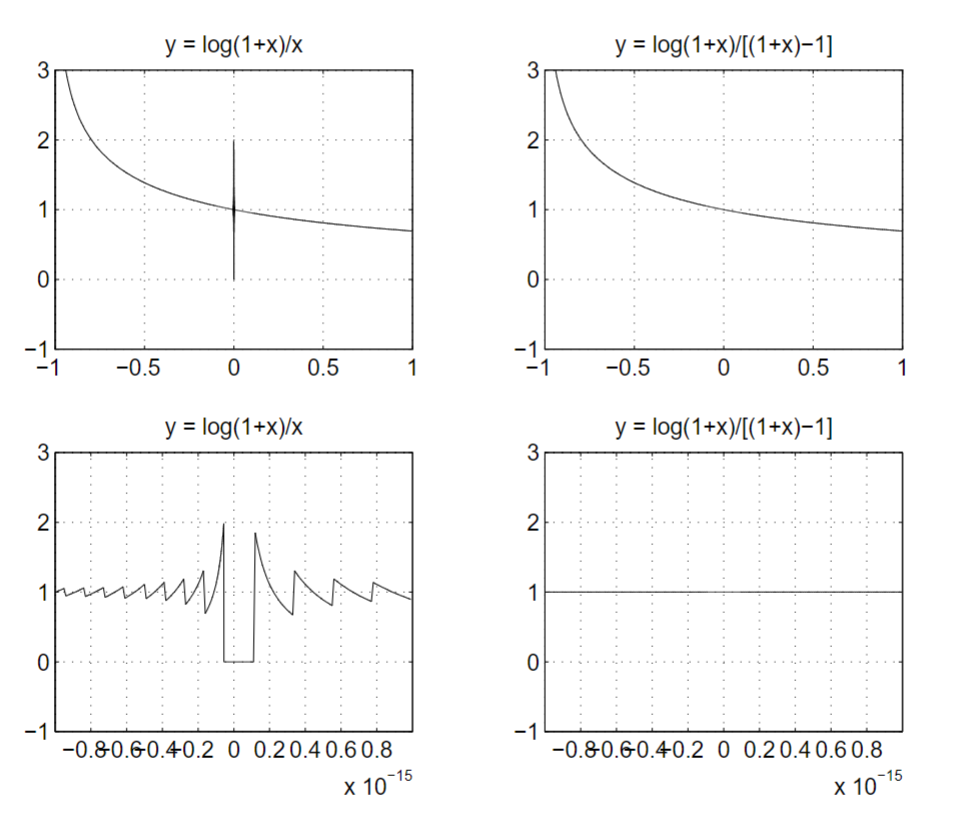
\includegraphics{figure/question1_9}
    \label{fig:1.9}
\end{figure}

\pf

\subsection{}
Show that, barring overflow or underflow, $\fl(\sum^d
_{i=1} x_i y_i) = \sum^d_{i=1} x_i y_i(1 + \delta_i)$, where $\abs{\delta_i} \le d\epsilon$. 
Use this to prove the
following fact. Let $A^{m\times n}$ and $B^{n\times p}$ be matrices, and compute their product
in the usual way. Barring overflow or underflow show that $\abs{\fl(A\cdot B) - A\cdot B} \le
n \cdot \epsilon \cdot \abs{A} \cdot \abs{B}$. Here the absolute value of a matrix $\abs{A}$ means the matrix with
entries $(\abs{A})_{ij} = \abs{a_{ij}}$, and the inequality is meant componentwise.
The result of this question will be used in section 2.4.2, where we analyze
the roundoff errors in Gaussian elimination.

\pf

\subsection{}
Let $L$ be a lower triangular matrix and solve $Lx =
b$ by forward substitution. Show that barring overflow or underflow, the computed
solution $\hat{x}$ satisfies $(L + \delta L)\hat{x} = b$, where $\abs{\delta l_{ij}} \le n\epsilon\abs{l_{ij}}$, where $\epsilon$ is the
machine precision. This means that forward substitution is backward stable.
Argue that backward substitution for solving upper triangular systems satisfies
the same bound.
The result of this question will be used in section 2.4.2, where we analyze
the roundoff errors in Gaussian elimination.

\pf

\subsection{}
In order to analyze the effects of rounding errors, 
we have used the following model (see equation (1.1)):
\begin{equation*}
    \fl(a\odot b) = (a \odot b)(1+\delta)
\end{equation*}
where $\odot$ is one of the four basic operations $+, -, *$, and $/$, and $|\delta| \le \epsilon$. 
To show
that our analyses also work for complex data, we need to prove an analogous
formula for the four basic complex operations. Now $\delta$ will be a tiny complex
number bounded in absolute value by a small multiple of $\epsilon$ . Prove that this
is true for complex addition, subtraction, multiplication, and division. Your
algorithm for complex division should successfully compute $a/a \approx 1$, where
$|a|$ is either very large (larger than the square root of the overflow threshold)
or very small (smaller than the square root of the underflow threshold). Is it
true that both the real and imaginary parts of the complex product are always
computed to high relative accuracy?

\pf

\subsection{}
Prove lemma 1.3.:~
Let $\mathcal{B}  = \mathbb{R}^n$ (or $\mathbb{C}^n$) and $\langle ·, ·\rangle$ be an inner product. Then there
is an $n$-by-$n$ \,s.p.d. (h.p.d.) matrix $A$ such that  $\langle x, y\rangle = y^T Ax \,(y^*Ax)$. 
Conversely, if $A$ is s.p.d (h.p.d.), then $y^TAx\,(y^*Ax)$ is an inner product.

\pf

\subsection{}
Prove lemma 1.5: $\forall x \in \Real^n,$\\ 
\begin{eqnarray*}
    \norm{x_2}& \leq\norm{x}_1\leq \sqrt{n}\norm{x_2}_2,\\ 
    \norm{x_2}_{\infty} & \leq\norm{x_2}_2\leq \sqrt{n}\norm{x_2}_{\infty},\\ 
    \norm{x_2}_{\infty} & \leq\norm{x_2}_1\leq n\norm{x_2}_{\infty}
\end{eqnarray*}.

\pf

\subsection{}
Prove lemma 1.6.: An operator norm is a matrix norm.

\pf

\subsection{}
Prove all parts except 7 of Lemma 1.7. Hint for
part 8: Use the fact that if $X$ and $Y$ are both $n$-by-$n$, then $XY$ and $YX$ have
the same eigenvalues. Hint for part 9: Use the fact that a matrix is normal if
and only if it has a complete set of orthonormal eigenvectors.

\pf

\subsection{}
We mentioned that on a Cray machine
the expression $\arccos(x/\sqrt{x^2 + y^2})$ caused an error, because roundoff caused
$(x/\sqrt{x^2 + y^2})$ to exceed 1. Show that this is impossible using IEEE arithmetic,
barring overflow or underflow. Hint: You will need to use more than the simple
model $fl(a \odot b)=(a \odot b)(1 + \delta)$ with $|\delta|$ small. Think about evaluating $\sqrt{x^2}$,
and show that, barring overflow or underflow, $fl(\sqrt{x^2}) = x$ exactly; in numerical
experiments done by A. Liu, this failed about 5\% of the time on a Cray YMP.
You might try some numerical experiments and explain them. Extra credit:
Prove the same result using correctly rounded decimal arithmetic. (The proof
is different.) This question is due to W. Kahan, who was inspired by a bug in
a Cray program of J. Sethian.

\pf

\subsection{}
Suppose $a$ and $b$ are normalized IEEE double precision floating point numbers, and consider the following algorithm, running
with IEEE arithmetic:

\begin{align*}
    &\text{IF} (\abs{a}<\abs{b}), \text{swap} a \text{and} b\\
    &s_1 = a+ b\\
    &s_2 = (a-s_1) + b
\end{align*}

Prove the following facts:
\begin{itemize}
    \item[1.] Barring overflow or underflow, the only roundoff error committed in running the algorithm is computing $s_1 = fl(a + b)$. In other words, both
    subtractions $s_1 - a$ and $(s_1 - a) - b$ are computed exactly.
    \item[2.] $s_1 +s_2 = a+b$,exactly. This means that $s_2$ is actually the roundoff error
    committed when rounding the exact value of $a + b$ to get $s_1$.
\end{itemize}
Thus, this program in effect simulates quadruple precision arithmetic, representing the true sum $a + b$ as the higher-order bits $(s_1)$ and the lower-order
bits $(s_2)$.
Using this and similar tricks in a systematic way, it is possible to effi-
ciently simulate all four basic floating point operations in arbitrary precision
arithmetic, using only the underlying floating point instructions and no “bit-
fiddling” [202]. $128$-bit arithmetic is implemented this way on the IBM RS6000
and Cray (but much less efficiently on the Cray, which does not have IEEE
arithmetic).

\pf

\section{}

\subsection{}
Using  your  favorite  World  Wide  Web  browser,  go toNETLIB (http://www.netlib.org), and answer the following questions

\begin{enumerate}
    \item  You need a Fortran subroutine to compute the eigenvalues and eigenvec-tors of real symmetric matrices in double precision.  Find one using theAttribute/Value database search on the NETLIB repository.  Report thename and URL of the subroutine as well as how you found it.
    \item   Using the Performance Database Server, find out the current world speedrecord for solving $100$-by-$100$ dense linear systems using Gaussian elimination.  What is the speed in Mflops, and which machine attained it?  Dothe same for $1000$-by-$1000$  dense linear  systems and "big as you want" dense linear systems.  Using the same database, find out how fast your work station  can  solve  $100$-by-$100$  dense  linear  systems.   Hint:  Look  atthe LINPACK benchmark. 
\end{enumerate}

\pf

\subsection{}
Consider solving $AX = B$ for $X$, where $A$ is $n$-by-$n$, and $X$ and $B$ are $n$-by-$m$. 
There are two obvious algorithms. The first algorithm factorizes $A = PLU$ using Gaussian elimination and then solves for
each column of $X$ by forward and back substitution. The second algorithm
computes $A^{-1}$ using Gaussian elimination and then multiplies $X = A^{-1}B$. Count the number of flops required by each algorithm, and show that the first one requires fewer flops.

\pf

\subsection{}
Let $\|\cdot\|$ be the two-norm. Given a nonsingular
matrix $A$ and a vector $b$, show that for sufficiently small $\|\delta A\|$ , there are nonzero
$\delta A$ and $\delta b$ such that inequality (2.2) is an equality. This justifies calling 
$\kappa(A) = \|A^{-1}\|\dot \|A\|$ the condition number of $A$. 
Hint: Use the ideas in the proof of Theorem 2.1.

\pf

\subsection{}
Show that bounds (2.7) and (2.8) are attainable.(\cref{fig:2_6})

\begin{figure}[h]
    \centering
    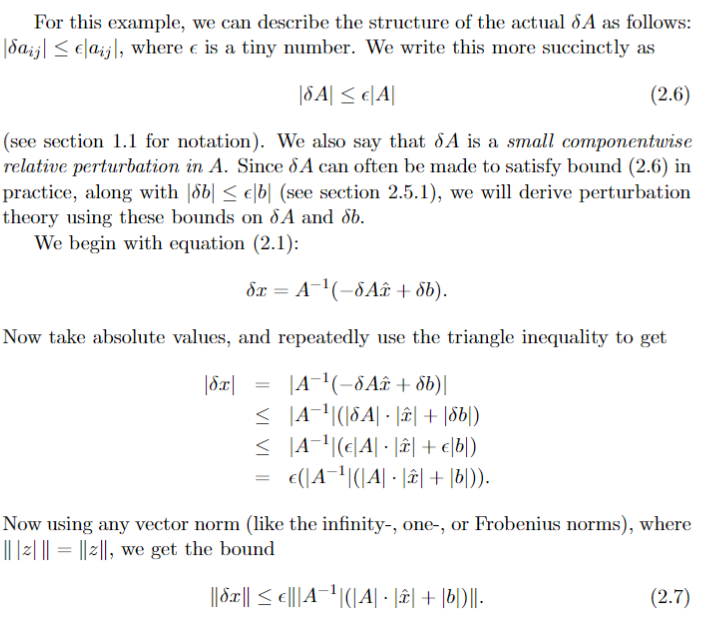
\includegraphics[width=12cm,height=10cm]{figure/question2_6_1.png}
    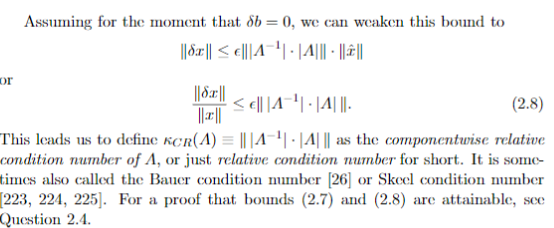
\includegraphics{figure/question2_6_2.png}
    \caption{question 2.6.}
    \label{fig:2_6}
\end{figure}

\pf

\subsection{}
Prove Theorem 2.3. Given the residual $r = A\hat{x} - b$,
use Theorem 2.3 to show that bound (2.9) is no larger than bound (2.7). This
explains why LAPACK computes a bound based on (2.9), as described in
section 2.4.4.

\subsection{}
Prove Lemma 2.2.

Let $P$,$P_1$,and $P_2$ be $n$-by-$n$ permutation matrices and $X$ be an $n$-by-$n$ matrix.  Then
\begin{enumerate}
    \item $PX$ is the same as $X$ with its rows permuted. $XP$ is the same as $X$ with its columns permuted.
    \item $p^{-1} = P^\top$.
    \item $\det P = \pm 1$.
    \item $P_1 \cdot P_2$ is also a permutation matrix.
\end{enumerate}

\pf

\subsection{}
If $A$ is a nonsingular symmetric matrix and
has the factorization $A = LDM^T$ , where $L$ and $M$ are unit lower triangular
matrices and $D$ is a diagonal matrix, show that $L = M$.

\pf

\subsection{}
Consider the following two ways of solving a 2-by-2
linear system of equations:
\begin{equation*}
    Ax =  \left[
    \begin{matrix}
    a_{11} & a_{12} \\
    a_{21} & a_{22} 
    \end{matrix} \right]
    \cdot \left[
    \begin{matrix}
        x_{1} \\
        x_{2} 
    \end{matrix} \right]
    = \left[
    \begin{matrix}
        b_{1} \\
        b_{2} 
    \end{matrix} \right]
    = b
\end{equation*} 

Algorithm 1. Gaussian elimination with partial pivoting (GEPP).

Algorithm 2. Cramer's rule.

Show by means of a numerical example that Cramer's rule is not backward
stable. Hint: Choose the matrix nearly singular and $[b_1 b_2]^\top \approx [a_{12} a_{22}]^\top$.
What does backward stability imply about the size of the residual? Your
numerical example can be done by hand on paper 
(for example, with four-decimal-digit floating point), 
on a computer, or a hand calculator.

\pf

\subsection{}
Let $B$ be an $n$-by-$n$ upper bidiagonal matrix, i.e.,
nonzero only on the main diagonal and first superdiagonal. Derive an algorithm
for computing $\kappa_{\infty}(B) := \|B\|_{\infty} \|B^{-1}\|_{\infty}$
exactly (ignoring roundoff ). In other
words, you should not use an iterative algorithm such as Hager's estimator.
Your algorithm should be as cheap as possible; it should be possible to do using
no more than $2n - 2$ additions, $n$ multiplications, $n$ divisions, $4n - 2$ absolute
values, and $2n - 2$ comparisons. (Anything close to this is acceptable.) 

\pf

\subsection{}
Let $A$ be $n$-by- $n$. Show that $\left\|A^{\top} A\right\|_2=\|A\|_2^2$ and $\kappa_2\left(A^{\top} A\right)=\kappa_2(A)^2$.

\pf

\subsection{}
Let $A$ be symmetric and positive definite. Show that $\left|a_{ij}\right|<\left(a_{i i} a_{j j}\right)^{1/2} .(i \neq j).$

\pf

\subsection{}
Show that if
\[Y = \begin{pmatrix}
I_n & Z \\
0& I_n
\end{pmatrix},\]
then $\kappa_{F(Y)}=\|Y\|_F\left\|Y^{-1}\right\|_F=2n+\|Z\|_F^2$.

\pf

\subsection{}
In this question we will ask how to solve $B y=c$ given a fast way to solve $A x=b$, where $A-B$ is "small" in some sense.
\begin{enumerate}
    \item Prove the Sherman-Morrison formula: Let $A$ be nonsingular, $u$ and $v$ be column 
    vectors, and $A+u v^{\top}$ be nonsingular. Then
    $ \left(A+u v^{\top}\right)^{-1}=A^{-1}-\left(A^{-1} u v^{\top} A^{-1}\right) /\left(1+v^{\top} A^{-1} u\right) .$ \\

    More generally, prove the Sherman-Morrison-Woodbury formula: Let $U$ and $V$ be $n$ by- $k$ rectangular matrices, were $k \leq n$ and $A$ is $n$-by- $n$. Then $T=I+V^{\top} A^{-1} U$ 
    is nonsingular if and only if $A+U V^{\top}$ is nonsingular, in which case
    $\left(A+U V^{\top}\right)^{-1}=A^{-1}-A^{-1} U T^{-1} V^{\top} A^{-1} .$
    \item If you have a fast algorithm to solve $A x=b$, show how to build a fast solver for $B y=c$, where $B=A+u v^{\top}$.
    \item Suppose that $\|A-B\|$ is "small" and you have a fast algorithm for solving $A x=b$. Describe an iterative scheme for solving $B y=c$. How fast do you expect your algorithm to converge? Hint: Use iterative refinement.
\end{enumerate}

\pf

\subsection{Programming,ommitted}
\subsection{Programming,ommitted}
\subsection{}
Show how to reorganize the Cholesky algorithm (Algorithm 2.11) to do most of its operations using Level $3$ BLAS. Mimic Algorithm 2.10.

\pf

\subsection{}
Let
\begin{equation*}
    A = \begin{pmatrix}
        A_{11} & A_{12} \\
        A_{21} & A_{22}
    \end{pmatrix},
\end{equation*}
where $A_{11}$ is $k$-by-$k$ and nonsingular. Then $S=A_{22}-A_{21} A_{11}^{-1} A_{12}$ is called the Schur complement of $A_{11}$ in $A$, or just Schur complement for short.\par
\begin{enumerate}
    \item Show that after $k$ steps of Gaussian elimination without pivoting, $A_{22}$ has been overwritten by $S$.
    \item Suppose $A=A^T, A_{11}$ is positive definite and $A_{22}$ is negative definite $\left(-A_{22}\right.$ is positive definite). Show that $A$ is nonsingular, that Gaussian elimination 
    without pivoting will work in exact arithmetic, but (by means of a 2-by-2 example) 
    that Gaussian elimination without pivoting may be numerically unstable.
\end{enumerate}

\pf

\subsection{}
Matrix $A$ is called column diagonally dominant, or diagonally dominant for short, if
\[\left|a_{i i}\right|>\sum_{j \neq i}\left|a_{j i}\right|.\]
\begin{enumerate}
    \item Show that $A$ is nonsingular. Hint: Use Gershgorin's theorem
    \item Show that Gaussian elimination with partial pivoting does not actually 
    permute any rows, i.e., that is identical to GEWP. Hint: Show that after one 
    step of Gaussian elimination, 
    the trailing submatrix, the Schur complement of $a_{11}$ in $a$ , is still diagonally dominant.
\end{enumerate}

\pf

\subsection{}
Given an $n$-by-$n$ nonsingular matrix $A$, how do you efficiently solve the following problems, 
using Gaussian elimination with partial pivoting?
\begin{enumerate}
    \item Solve the linear system $A^k x = b$, where $k$ is a positive integer.
    \item Compute $\alpha=c^{\top} A^{-1} b$.
    \item Solve the matrix equation $AX=B$, where $B$ is $n$-by-$m$.
\end{enumerate}

\pf

\subsection{}

Prove that Strassen's algorithm (Algorithm 2.8) 
correctly multiplies $n$-by-$n$ matrices, where $n$ is a power of 2.

\pf

\section{}

\subsection{}
Show that the two variations of Algorithm 3.1, CGS
and MGS, are mathematically equivalent by showing that the two formulas for
rji yield the same results in exact arithmetic.

\pf

\subsection{}
This question will illustrate the difference in numerical
stability among three algorithms for computing the QR factorization
 of a matrix: 
\begin{itemize}
    \item Householder QR (Algorithm 3.2),
    \item CGS (Algorithm 3.1),
    \item MGS (Algorithm 3.1)
\end{itemize}
Obtain the Matlab program QRStability.m from
HOMEPAGE/Matlab/QRStability.m. This program generates random matrices
 with user-specified dimensions $m$ and $n$ and condition number $cnd$, computes
their QR decomposition using the three algorithms, and measures the accuracy
of the results. It does this with the residual $\frac{\norm{A - Q \cdot R}}{\norm{A}}$, which should be
around machine epsilon $\epsilon$ for a stable algorithm, and the orthogonality of Q
$\norm{Q^\top \cdot Q - I}$, which should also be around $\epsilon$. Run this program for small matrix
 dimensions (such as $m= 6$ and $n= 4$), modest numbers of random matrices
(samples$= 20$), and condition numbers ranging from $cnd= 1$ up to $cnd= 1015$.
Describe what you see. Which algorithms are more stable than others? See
if you can describe how large $\norm{Q^\top \cdot Q - I}$ can be as a function of choice of
algorithm, $cnd$ and $\epsilon$.

\pf

\subsection{}
Let $A$ be $m$-by-$n$, $m \ge n$, and have full rank.
\begin{itemize}
    \item Show that $\begin{pmatrix}
        I&A\\
        A^\top&0
    \end{pmatrix}\cdot\begin{pmatrix}
        r\\x
    \end{pmatrix} = \begin{pmatrix}
        b\\0
    \end{pmatrix}$ has a solution where $x$
    minimizes $\norm{Ax - b}_2$. One reason for this formulation is that we can
    apply iterative refinement to this linear system if we want a more accurate
    answer (see section 2.5).
    \item What is the condition number of the coefficient matrix, in
    terms of the singular values of $A$? Hint: Use the SVD of $A$.
    \item Give an explicit expression for the inverse of the cofficient
    matrix, as a block $2$-by-$2$ matrix. Hint: Use $2$-by-$2$ block Gaussian elimination. Where have we previously seen the $(2,1)$ block entry?
    \item Show how to use the QR decomposition of $A$ to implement an
    iterative refinement algorithm to improve the accuracy of $x$.
\end{itemize}

\pf

\subsection{}
Weighted least squares: If some components of $Ax-b$ 
are more important than others, we can weight them with a scale factor $d_i$ 
and solve the weighted least squares problem $\min \|D(A x-b)\|_2$ instead, 
where $D$ has diagonal entries $d_i$. More generally, recall that if $C$ is 
symmetric positive definite, then $\|x\|_C \equiv\left(x^T C x\right)^{1/2}$ 
is a norm, and we can consider minimizing $\|A x-b\|_C$. Derive the normal 
equations for this problem, 
as well as the formulation corresponding to the previous question.

\pf

\subsection{}
Let $A \in \mathbb{R}^{n \times n}$ 
be positive definite. Two vectors $u_1$ and $u_2$ are called $A$-orthogonal 
if $u_1^T A u_2=0$. If $U \in \mathbb{R}^{n \times r}$ and $U^T A U=I$, 
then the columns of $U$ are said to be $A$-orthonormal. 
Show that every subspace has an $A$-orthonormal basis.

\pf

\subsection{}
Let $A$ have the form
$A =\begin{pmatrix}
    R\\S
\end{pmatrix}$,
where $R$ is $n$-by-$n$ and upper triangular, and $S$ is $m$-by-$n$ and dense. Describe
an algorithm using Householder transformations for reducing $A$ to upper triangular form. 
Your algorithm should not “fill in” the zeros in $R$ and thus require
fewer operations than would Algorithm 3.2 applied to $A$.

\pf

\subsection{}
If $A=R+u v^T$, where $R$ is an upper triangular 
matrix, and $u$ and $v$ are column vectors, describe an efficient algorithm to 
compute the QR decomposition of $A$. Hint: Using Givens rotations, your 
algorithm should take $O\left(n^2\right)$ operations. 
In contrast, Algorithm $3.2$ would take $O\left(n^3\right)$ operations.

\pf

\subsection{}
Let $x \in \mathbb{R}^n$ and let $P$ be a Householder matrix such 
that $P x=\pm\|x\|_2e_1$. Let $G_{1,2}, \ldots, G_{n-1, n}$ be Givens rotations, 
and let $Q=G_{1,2} \cdots G_{n-1, n}$. Suppose $Q x=\pm\|x\|_2e_1$. 
Must $P$ equal $Q$ ? (You need to give a proof or a counterexample.)

\pf

\subsection{}
Let $A$ be $m$-by-$n$, with SVD $A = U\Sigma V^T$ .
Compute the SVDs of the following matrices in terms of $U, \Sigma$, and $V$:
\begin{enumerate}
    \item $(A^TA)^{-1},$
    \item $(A^TA)^{-1}A^T,$
    \item $A(A^TA)^{-1},$
    \item $A(A^TA)^{-1}A^T.$
\end{enumerate}

\pf

\subsection{}
Let $A_k$ be a best rank-$k$ approximation
 of the matrix $A$, as defined in Part 9 of Theorem 3.3. Let $\sigma_i$ be the $i$-th
singular value of $A$. Show that $A_k$ is unique if $\sigma_k > \sigma_{k+1}$.

\pf

\subsection{}
Let $A$ be $m$-by-$n$. Show that $X = A^\dagger $ (the
Moore-Penrose pseudoinverse) minimizes $\|AX -I\|_F$  over all $n$-by-$m$ matrices
$X$. What is the value of this minimum?

\pf

\subsection{}
Let $A, B$, and $C$ be matrices with dimensions such that the product $A^T CB^T$ 
is well defined. Let $\mathcal{X}$ be the set of
matrices $X$ minimizing $ \|AXB - C\|_F$ , and let $X_0$ be the unique member of $\mathcal{X}$
minimizing $\|X\|_F$ . Show that $X_0 = A^\dagger CB^\dagger\|$. 
Hint: Use the SVDs of $A$ and $B$.

\pf

\subsection{}
Show that the Moore-Penrose pseudoinverse of A satisfies the following identities:
\begin{enumerate}
    \item $AA^+A = A$,
    \item $A^+AA^+ = A^+$,
    \item $A^+A = (A^+A)^\top$,
    \item $AA^+ = (AA^+)^\top$.
\end{enumerate}

\pf

\subsection{}
Prove part4 of Theorem $3.3$ : 
Let $H=\left[\begin{array}{cc}0& A^T \\ A &0\end{array}\right]$,
where $A$ is square and $A=U \Sigma V^T$ is its SVD. Let 
$\Sigma=$ $\operatorname{diag}\left(\sigma_1, \ldots, \sigma_n\right), U=\left[u_1, \ldots, u_n\right]$, 
and $V=\left[v_1, \ldots, v_n\right]$. Prove that the $2n$ 
eigenvalues of $H$ are $\pm \sigma_i$, with corresponding unit eigenvectors 
$\frac{1}{\sqrt{2}}\left[\begin{array}{c}v_i \\ \pm u_i\end{array}\right]$. 
Extend to the case of rectangular $A$.

\pf

\subsection{}
Let $A$ be $m$-by-$n$, $m<n$, and of full rank. Then
$\min \|Ax - b\|_2$ is called an underdetermined least squares problem. Show that
the solution is an $(n - m)$-dimensional set. Show how to compute the unique
minimum norm solution using appropriately modified normal equations, QR
decomposition, and SVD.

\pf

\subsection{}
Prove Lemma 3.1.

Let $P$ be an exact Householder (or Givens) transformation, and $\tilde{P}$ be its floating point approximation.  Then
\begin{equation*}
    \fl(\tilde{P}A) = P(A+E),\quad \norm{E}_2 = \Order(\epsilon)\norm{A}_2,
\end{equation*}
and
\begin{equation*}
    \fl(A\tilde{P}) = (A+F)P,\quad \norm{F}_2 = \Order(\epsilon)\norm{A}_2.
\end{equation*}
Sketch  of  Proof: Apply  the usual  formula $\fl(a\odot b)=(a\odot b)(1 +\epsilon)$ to the formulas for computing and applying $\tilde{P}$.  See Question 3.16.

\pf

\subsection{}
In section 2.6.3, we showed how to reorganize Gaussian
 elimination to perform Level $2$ BLAS and Level $3$ BLAS as each step in
order to exploit the higher speed of these operations. In this problem, we will
show how to apply a sequence of Householder transformations using Level $2$
and Level $3$ BLAS.

\begin{enumerate}
    \item Let $u_1, \ldots , u_b$ be a sequence of vectors of dimension $n$, where ${\norm{u_i}}_2 = 1$
    and the first $i - 1$ components of $u_i$ are zero. Let $P = P_b \cdot P_{b-1} \cdots P_1$,
    where $P_i = I - 2u_iu^\top_i$ is a Householder transformation. Show that there
    is a $b$-by-$b$ lower triangular matrix $T$ such that $P = I - UTU^\top$ , where
    $U = [u_1, \ldots , u_b]$. In particular, provide an algorithm for computing the
    entries of $T$ . This identity shows that we can replace multiplication by $b$
    Householder transformations $P_1$ through $P_b$ by three matrix multiplications by $U$,
    $T$ , and $U^\top$(plus the cost of computing $T$).
    \item Let House($x$) be a function of the vector $x$ which returns a unit vector $u$
    such that $(I - 2uu^\top )x = \norm{x}_2e_1$; we showed how to implement House($x$)
    in section 3.4. Then Algorithm 3.2 for computing the QR decomposition
    of the $m$-by-$n$ matrix $A$ may be written as
    \begin{align*}
        &\text{for}\; i = 1 : m\\
        &u_i = \text{House}(A(i : m, i))\\
        &P_i = I - 2u_iu^\top_i\\
        &A(i : m, i : n) = P_i A(i : m, i : n)\\
        &\text{endfor}
    \end{align*}
    Show how to implement this in terms of the Level $2$ BLAS in an efficient
    way (in particular, matrix-vector multiplications and rank-$1$ updates).
    What is the floating point operation count? (Just the high-order terms
    in n and m are enough.) It is sufficient to write a short program in the
    same notation as above (although trying it in Matlab and comparing
    with Matlab's own QR factorization are a good way to make sure that
    you are right!).
    \item Using the results of step (1), show how to implement QR decomposition
    in terms of Level $3$ BLAS. What is the operation count? This technique is
    used to accelerate the QR decomposition, just as we accelerated Gaussian
    elimination in section 2.6. It is used in the LAPACK routine $sgeqrf$
    
\end{enumerate}

\pf

\subsection{}
It is often of interest to solve constrained least
squares problems, where the solution $x$ must satisfy a linear or nonlinear constraint
 in addition to minimizing $\norm{Ax - b}_2$. We consider one such problem
here. Suppose that we want to choose $x$ to minimize  in addition to minimizing $\norm{Ax - b}_2$. We consider one such problem
subject to
the linear constraint $Cx = d$. Suppose also that $A$ is $m$-by-$n$, $C$ is $p$-by-$n$,
and $C$ has full rank. We also assume that $p \le n$ (so $Cx = d$ is guaranteed to be consistent)
and $n \le m + p$ (so the system is not underdetermined). Show
that there is a unique solution under the assumption that $\begin{pmatrix}
    A\\C
\end{pmatrix}$ has full column
rank. Show how to compute $x$ using two QR decompositions and some matrix-vector
multiplications and solving some triangular systems of equations. Hint:
Look at LAPACK routine sgglse and its description in the LAPACK manual
[10] (NETLIB/lapack/lug/lapack lug.html)

\pf

\subsection{}
Write a program (in Matlab or any
other language) to update a geodetic database using least squares, as described
in Example 3.3. Take as input a set of “landmarks,” their approximate coordinates $(x_i, y_i)$,
and a set of new angle measurements $\theta_j$ and distance measurements
$L_{ij}$ . The output should be corrections $(\delta x_i, \delta y_i)$ for each landmark, an
error bound for the corrections, and a picture (triangulation) of the old and
new landmarks.

\subsection{}
Prove Theorem 3.4.

Suppose that $A$ is $m$-by-$n$ with $m\ge n$ and has full rank.  
Suppose that $x$ minimizes $\norm{Ax-b}_2$. Let $r=b-Ax$ be the residual.  
Let $\tilde{x}$ minimize $\norm{(A+\delta A)\tilde{x}-(b+\delta b)}_2$.   
Assume
\begin{equation*}
    \epsilon := \max (\frac{\norm{\delta A}_2}{\norm{A}_2},\frac{\norm{\delta b}_2}{\norm{b}_2}) < \frac{1}{\kappa_2(A)} = \frac{\sigma_{\min}(A)}{\sigma_{\min}(A)}.
\end{equation*}
Then
\begin{equation*}
    \frac{\norm{\tilde{x}-x}_2}{\norm{x}_2}\le \epsilon \cdot \{\frac{2\cdot\kappa_2(A)}{\cos\theta} + \tan\theta\cdot\kappa_2^2(A)\} + \Order(\epsilon^2) \equiv \epsilon\cdot\kappa_{LS} + \Order(\epsilon^2).
\end{equation*}
where $\sin\theta = \frac{\norm{r}_2}{\norm{b}_2}$. In other words, $\theta$ 
is the angle  between  the  vectors $b$ and $Ax$ and measures whether  the 
residual  norm $\norm{r}_2$ is large(near$\norm{b}$) or  small(near $0$). $\kappa_{LS}$ is the condition number for the least squares problem.

\pf

\subsection{}
Redo Example 3.1, using a rank-deficient least
squares technique from section 3.5.1. Does this improve the accuracy of the
high-degree approximating polynomials?

\pf

\section{}


\subsection{}
Let $A$ be defined  as  in  equation  (4.1).    Show  that $\det(A)=\prod_{i=1}^b\det(A_{ii})$  and  then  that  $\det(A- \lambda I)=\prod_{i=1}^b\det(A_{ii}-\lambda I)$. Conclude that the set of eigenvalues of $A$ is the union of the sets of eigenvalues of $A_{11}$ through $A_{bb}$.

\pf

\subsection{}
Suppose that $A$ is normal; i.e.,$AA^\dag=A^\dag A$. Show that if $A$ is also triangular, it must be diagonal.  Use this to show that an $n$-by-$n$ matrix is normal if and only if it has $n$ orthonormal eigenvectors. Hint:  Show that $A$ is normal if and only if its Schur form is normal.

\pf

\subsection{}
Let $\lambda$ and $\mu$ be distinct eigenvalues of $A$, let $x$ be a right eigenvector for $\lambda$, and let $y$ be a left eigenvecctor for $\mu$.  Show that $x$ and $y$ are orthogonal.

\pf

\subsection{}
Suppose $A$ has  distinct  eigenvalues.   Let 
\begin{equation*}
    f(z) = \sum_{i=-\infty}^{+\infty}a_i z^i
\end{equation*}
be a function which is defined at the eigenvalues of $A$. Let
\begin{equation*}
    Q^\dag A Q = T
\end{equation*}
be the Schur form of $A$(so $Q$ is unitary and $T$ upper triangular).
\begin{enumerate}
    \item  Show  that $f(A)=Qf(T)Q^\dag$.   Thus  to  compute $f(A)$  it  suffices  to  be able  to  compute $f(T)$.   In  the  rest  of  the  problem  you  will  derive  asimple recurrence formula for $f(T)$.
    \item  Show that $(f(T))_{ii}=f(T_{ii})$ so that the diagonal of $f(T)$ can be computedfrom the diagonal of $T$.
    \item  Show that $Tf(T)=f(T)T$.
    \item From  the  last  result,  show  that  theith  superdiagonal  of $f(T)$ can be computed  from  the  $(i-1)$-st  and  earlier  subdiagonals.   Thus,  startingat the diagonal of $f(T)$, we can compute the first superdiagonal, second super diagonal, and so on.
\end{enumerate}

\pf

\subsection{}
Let $A$ be a square matrix. Apply either Question 4.4
to the Schur form of $A$ or equation (4.6) to the Jordan form of $A$ to conclude
that the eigenvalues of $f(A)$ are $f(\lambda_i)$, where the $\lambda_i$ are the eigenvalues of $A$.
This result is called the spectral mapping theorem.
This question is used in the proof of Theorem 6.5 and section 6.5.6.

\pf

\subsection{}
In this problem we will show how to solve the
Sylvester or Lyapunov equation $AX - XB = C$, where $X$ and $C$ are $m$-by-$n$,
$A$ is $m$-by-$m$, and $B$ is $n$-by-$n$. This is a system of $mn$ linear equations for the
entries of $X$.
\begin{enumerate}
    \item Given the Schur decompositions of $A$ and $B$, show how $AX - XB = C$
    can be transformed into a similar system $A'Y - Y B' = C'$, where $A'$ and
    $B'$ are upper triangular.
    \item Show how to solve for the entries of $Y$ one at a time by a process analogous
     to back substitution. What condition on the eigenvalues of $A$ and
    $B$ guarantees that the system of equations is nonsingular?
    \item Show how to transform $Y$ to get the solution $X$.
\end{enumerate}

\pf

\subsection{}
Suppose that $T = \begin{pmatrix}A&C\\0&B\end{pmatrix}$  is in Schur form.
We want to find a matrix $S$ so that $S^{-1}T S =  \begin{pmatrix}A&0\\0&B\end{pmatrix}$. It turns out we can choose
$S$ of the form $\begin{pmatrix}I&R\\0&I\end{pmatrix}$. Show how to solve for $R$.

\pf

\subsection{}
Let $A$ be $m$-by-$n$ and $B$ be $n$-by-$m$. Show
that the matrices
\begin{equation*}
    \begin{pmatrix}
        AB&0\\B&0
    \end{pmatrix}
    \text{and}
    \begin{pmatrix}
        0&0\\B&BA
    \end{pmatrix}
\end{equation*}
are similar. Conclude that the nonzero eigenvalues of $AB$ are the same as
those of $BA$.

\pf

\subsection{}
Let $A$ be $n$-by-$n$ matrix with eigenvalues $\lambda_1, \ldots , \lambda_n$.
Show that
\begin{equation*}
    \sum_{i=1}^n\abs{\lambda_i}^2 = \min_{\det(S) =0}\norm{S^{-1}AS}^2_F.
\end{equation*}

\pf

\subsection{}
Let $A$ be $n$-by-$n$ matrix with eigenvalues $\lambda_1, \ldots , \lambda_n$.
\begin{enumerate}
    \item Show that $A$ can be written $A = H + S$, where $H = H^\dag$ is Hermitian
    and $S = -S^\dag$ is skew-Hermitian. Give explicit formulas for $H$ and $S$ in
    terms of $A$.
    \item Show that $\sum_{i=1}^n\abs{\mathcal{R}\lambda_i}^2\le \norm{H}_F^2$.
    \item Show that $\sum_{i=1}^n\abs{\mathcal{I}\lambda_i}^2\le \norm{S}_F^2$.
    \item Show that $A$ is normal iff $\sum_{i=1}^n\abs{\lambda_i}^2 = \norm{A}_F^2$.
\end{enumerate}

\pf

\subsection{}
Let $\lambda$ be a simple eigenvalue, and let $x$ and $y$ be right
and left eigenvectors. We define the spectral projection $P$ corresponding to $\lambda$
as $P = \frac{xy^\dag}{y^\dag x}$. Prove that $P$ has the following properties.
\begin{enumerate}
    \item $P$ is uniquely defined, even though we could use any nonzero scalar multiples
     of $x$ and $y$ in its definition.
    \item $P^2 = P$. (Any matrix satisfying $P^2 = P$ is called a projection matrix.)
    \item $AP = P A = \lambda P$ . (These properties motivate the name spectral projection,
     since $P$ “contains” the left and right invariant subspaces of $\lambda$.)
    \item $\norm{P}_2$ is the condition number of $\lambda$.
\end{enumerate}

\pf

\subsection{}
Let 
\begin{equation*}
    A = \begin{pmatrix}
        c&c\\0&b
    \end{pmatrix}.
\end{equation*} 
Show that the condition
numbers of the eigenvalues of $A$ are both equal to 
\begin{equation*}
    (1 + (\frac{c}{a-b})^2)1/2.
\end{equation*}
Thus, the condition number is large if the difference $a-b$ between the eigenvalues is small
compared to $c$, the offdiagonal part of the matrix.

\pf

\subsection{}
Let $A$ be a matrix, $x$ be a unit vector, $\mu$ be a scalar, and $r = Ax - \mu x$. Show that there is a matrix $E$
with $\norm{E}_F = \norm{r}_2$ such that $A + E$ has eigenvalue $\mu$ and eigenvector $x$.

\pf

\subsection{Programming,omitted}
\subsection{Programming,omitted}

\section{}

\subsection{}
Show that $A = B +iC$ is Hermitian if and only if
\begin{equation*}
    M = \begin{pmatrix}
        B&-C\\C&B
    \end{pmatrix}
\end{equation*}
is symmetric. Express the eigenvalues and eigenvectors of $M$ in terms of those
of $A$.

\pf

\subsection{}
Prove Corollary 5.1, using Weyl's theorem (Theorem 5.1) and part 4 of Theorem 3.3.

\pf

\subsection{}
Consider Figure 5.1. Consider the corresponding
contour plot for an arbitrary $3$-by-$3$ matrix $A$ with eigenvalues $\alpha_3 \le \alpha_2 \le \alpha_1$.
Let $C_1$ and $C_2$ be the two great circles along which $\rho(u, A) = \alpha_2$. At what
angle do they intersect?

\pf

\subsection{}
Use the Courant-Fischer minimax theorem (Theorem 5.2) to prove the Cauchy interlace theorem:
\begin{enumerate}
    \item Suppose that $A = \begin{pmatrix}
        H&b\\b^\top&u
    \end{pmatrix}$ is an $n$-by-$n$ symmetric matrix and $H$ is
    $(n - 1)$-by-$(n - 1)$. Let $\alpha_n \le \cdots \le \alpha_1$ be the eigenvalues of $A$ and
    $\theta_{n-1} \le \cdots\le \theta_1$ be the eigenvalues of H. Show that these two sets of
    eigenvalues interlace:
    \begin{equation*}
        \alpha_n\le\theta_{n-1}\le\cdots\le\theta_i\le\alpha_i\le\theta_{i-1}\le\alpha_{i-1}\le\cdots\le\theta_1\le\alpha_1.
    \end{equation*}
    \item Let $A = \ttmat{H}{b}{b^\top}{u}$ be \bymn{n}{n} and $H$ be \bymn{m}{n},  with eigenvalues $\theta_m \le\cdots \le \theta_1$.
    Show that the eigenvalues of $A$ and $H$ interlace in the sense
    that $\alpha_j+(n-m) \le \theta_j \le \alpha_j$ (or equivalently $\alpha_j \le \theta_{j-(n-m)} \le \alpha_{j-(n-m)}$).
\end{enumerate}

\pf

\subsection{}
Let $A = A^\top$ with eigenvalues $\alpha_1 \le \cdots \le \alpha_n$. Let
$H = H^\top$ with eigenvalues $\theta_1 \le \cdots \le \theta_n$. Let $A + H$ have eigenvalues 
$\lambda_1 \le \cdots \le \lambda_n$. Use the Courant-Fischer minimax theorem (Theorem 5.2) to show
that $\alpha_j + \theta_n \le \lambda_j \le \alpha_j + \theta_1$. If $H$ is positive definite, conclude that $\lambda_j > \alpha_j$ .
In other words, adding a symmetric positive definite matrix $H$ to another
symmetric matrix $A$ can only increase its eigenvalues.

This result will be used in the proof of Theorem 7.1.

\pf

\subsection{}
Let $A = \tmat{A_1}{A_2}$ be \bymn{n}{n}, where $A_1$ is \bymn{n}{m}
and $A_2$ is \bymn{n}{n-m}. Let $\sigma_1\ge\cdots\ge\sigma_n$ be the singular values of $A
\tau_1 \ge \cdots\ge \tau_m$ be the singular values of $A_1$. Use the Cauchy interlace theorem
from Question 5.4 and part 4 of Theorem 3.3 to prove that $\sigma_j \ge \tau_j \ge \sigma_{j+n-m}$.

\pf

\subsection{}
Let $q$ be a unit vector and $d$ be any vector orthogonal to $q$. 
Show that $\norm{(q + d)q^\top - I}_2 = \norm{q + d}_2$. (This result is used in the
proof of Theorem 5.4.)

\pf

\subsection{}
Formulate and prove a theorem for singular vectors
analogous to Theorem 5.4.

\pf

\subsection{}
Prove bound (5.6) from Theorem 5.5.

\pf

\subsection{}
Prove bound (5.7) from Theorem 5.5.

\pf

\subsection{}
Suppose $\theta = \theta_1 +\theta_2$, where all three angles lie between
$0$ and $\frac{\pi}{2}$. Prove that 
\begin{equation*}
    \frac{\sin 2\theta}{2} \le \frac{\sin 2\theta_1 + \sin 2\theta_2}{2}.
\end{equation*}
This result is used in the proof of Theorem 5.7.

\pf

\subsection{}
Prove Corollary 5.2. Hint: Use part 4 of Theorem 3.3.

\pf

\subsection{}
Let $A$ be a symmetric matrix. Consider running
shifted QR iteration (Algorithm 4.5) with a Rayleigh quotient shift ($\sigma_i = a_{nn}$)
at every iteration, yielding a sequence $\sigma_1, \sigma_2, \ldots$ of shifts. Also run Rayleigh
quotient iteration (Algorithm 5.1), starting with $x_0 = [0, \ldots, 0, 1]^\top$ , yielding
a sequence of Rayleigh quotients $\rho_1, \rho_2, \ldots$. Show that these sequences are
identical: $\sigma_i = \rho_i$ for all $i$. This justifies the claim in section 5.3.2 that shifted
QR iteration enjoys local cubic convergence.

\pf

\subsection{}
Prove Lemma 5.1.

\pf

\subsection{}
Prove that if 
\begin{equation*}
    t(n) = 2t(\frac{n}{2}) + cn^3 + O(n^2),
\end{equation*} 
then
\begin{equation*}
    t(n) \approx c\frac{4}{3}n^3.
\end{equation*} This justifies the complexity analysis of the divide-and-conquer
algorithm (Algorithm 5.2).

\pf

\subsection{}
Let $A = D + \rho uu^\top$ , where $D = \text{diag}(d_1, \ldots , d_n)$ and
$u = [u_1, \ldots , u_n]^\top$ . Show that if $d_i = d_{i+1}$ or $u_i = 0$, then $d_i$ is an eigenvalue
of $A$. If $u_i = 0$, show that the eigenvector corresponding to $d_i$ is $e_i$, the
$i$-th column of the identity matrix. Derive a similarly simple expression when
$d_i = d_{i+1}$. This shows how to handle deflation in the divide-and-conquer
algorithm, Algorithm 5.2.

\pf

\subsection{}
Let $\psi$ and $\psi'$ be given scalars. Show how to compute
scalars $c$ and $\hat{c}$ in the function definition
\begin{equation*}
    h(\lambda) = \hat{c} + \frac{c}{d-\lambda}
\end{equation*} so that at $\lambda = \xi$,
$h(\xi) = \psi$, and $h'(\xi) = \psi'$. This result is needed to derive the secular equation
solver in section 5.3.3.

\pf

\subsection{}
Use the SVD to show that if $A$ is an \bymn{m}{n} real matrix with $m \ge n$, then there exists an \bymn{m}{n} matrix $Q$ with
orthonormal columns $(Q\top Q = I)$ and an \bymn{n}{n} positive semidefinite matrix $P$
such that $A = QP$. This decomposition is called the polar decomposition of $A$,
because it is analogous to the polar form of a complex number $z = e^{i\arg(z)} \cdot\abs{z}$.
Show that if $A$ is nonsingular, then the polar decomposition is unique.

\pf

\subsection{}
Prove Lemma 5.5.

\pf

\subsection{}
Prove Lemma 5.7.

\pf

\subsection{}

Prove Theorem 5.13. Also, reduce the exponent $4n -2$ in Theorem 5.13 to $2n - 1$. Hint: In Lemma 5.7, multiply $D_1$ and divide $D_2$
by an appropriately chosen constant.

\pf

\subsection{}
Prove that Algorithm 5.13 computes the SVD of
$G$, assuming that $G^\top G$ converges to a diagonal matrix.

\pf

\subsection{}
Let $A$ be an $n$-by-$n$ symmetric positive definite matrix with Cholesky decomposition $A = LL^T$, and let $\hat{L}$ be the Cholesky factor computed in floating point arithmetic. In this question we will bound the relative error in the (squared) singular values of $\hat{L}$ as approximations of the eigenvalues of $A$. Show that $A$ can be written as $A = DAD$, where $D = \mathrm{diag}(a_{1/2}^1, \ldots, a_{n/n}^n)$ and $a_{ii} = 1$ for all $i$. Write $L = DX$. Show that $\kappa^2(X) = \kappa(A)$. Using bound (2.16) for the backward error $\delta A$ of Cholesky $A + \delta A = \hat{L}\hat{L}^T$, show that one can write $\hat{L}^T\hat{L} = Y^TY$ where $\|Y^TY - I\|_2 \leq O(\epsilon)\kappa(A)$. Use Theorem 5.6 to conclude that the eigenvalues of $\hat{L}^T\hat{L}$ and of $L^T L$ differ relatively by at most $O(\epsilon)\kappa(A)$. Then show that this is also true of the eigenvalues of $\hat{L}^T\hat{L}$ and $L^TL$. This means that the squares of the singular values of $\hat{L}$ differ relatively from the eigenvalues of $A$ by at most $O(\epsilon)\kappa(A) = O(\epsilon)\kappa^2(L)$.

\pf

\subsection{}
This question justifies the stopping criterion for one-sided Jacobi's method for the SVD (Algorithm 5.13). Let $A = G^TG$, where $G$ and $A$ are $n$-by-$n$. Suppose that $|a_{jk}| \leq \epsilon \sqrt{a_{jj} a_{kk}}$ for all $j = k$. Let $\sigma_n \leq \cdots \leq \sigma_1$ be the singular values of $G$, and $\alpha_2^2 \leq \cdots \leq \alpha_1^2$ be the sorted diagonal entries of $A$. Prove that $|\sigma_i - \alpha_i| \leq n\epsilon|\alpha_i|$ so that the $\alpha_i$ equal the singular values to high relative accuracy. Hint: Use Corollary 5.2.

\pf

\subsection{}
In Question 4.15, you “noticed” that running QR for $m$ steps on a symmetric matrix, “flipping” the rows and columns, running for another $m$ steps, and flipping again got you back to the original matrix. (Flipping $X$ means replacing $X$ by $JXJ$, where $J$ is the identity matrix with its row in reverse order.) In this exercise we will prove this for symmetric positive definite matrices $T$ using an approach different from Corollary 5.4.

Consider $LR$ iteration (Algorithm 5.9) with a zero shift, applied to the symmetric positive definite matrix $T$ (which is not necessarily tridiagonal): Let $T = B_0^TB_0$ be the Cholesky decomposition, $T_1 = B_0B_0^T = B_1^TB_1$, and more generally $T_i = B_{i-1}B_{i-1}^T = B_i^TB_i$. Let $\hat{T}_i$ denote the matrix obtained from $T_0$ after $i$ steps of unshifted QR iteration; i.e., if $\hat{T}_i = Q_iR_i$ is the QR decomposition, then $\hat{T}_{i+1} = R_iQ_i$. In Lemma 5.6 we showed that $\hat{T}_i = T_2$; i.e., one step of QR is the same as two steps of LR.
\begin{enumerate}
    \item Show that $T_i = (B_{i-1}B_{i-2}\cdots B_0)^{-T}T_0(B_{i-1}B_{i-2}\cdots B_0)^T$.
    \item Show that $T_i = (B_{i-1}B_{i-2}\cdots B_0)T_0(B_{i-1}B_{i-2}\cdots B_0)^{-1}$.
    \item Show that $\hat{T}_0 = (B_iB_{i-1}\cdots B_0)^T(B_iB_{i-1}\cdots B_0)$ is the Cholesky decomposition of $\hat{T}_0$.
    \item Show that $\hat{T}^i_0 = (Q_0 \cdots Q_{i-2}Q_{i-1}) \cdot (R_{i-1}R_{i-2}\cdots R_0)$ is the QR decomposition of $\hat{T}^i_0$.
    \item Show that $\hat{T}^{2i}_0 = (R_{2i-1}R_{2i-2}\cdots R_0)^T(R_{2i-1}R_{2i-2}\cdots R_0)$ is the Cholesky decomposition of $\hat{T}^{2i}_0$.
    \item Show the result after $m$ steps of QR, flipping $m$ steps of QR, and flipping, is the same as the original matrix. Hint: Use the fact that the Cholesky factorization is unique.
\end{enumerate}

\pf

\subsection{}
Suppose that $x$ is an $n$-vector. Define the matrix $C$ by $c_{ij} = |x_i| + |x_j| - |x_i - x_j|$. Show that $C(x)$ is positive semidefinite.

\pf

\subsection{}
Let 

\[
A = \begin{pmatrix}
I & B^H \\
B & I
\end{pmatrix}
\]

with $\|B\|_2 < 1$. Show that 

\[
\|A\|_2 \|A^{-1}\|_2 = \frac{1 + \|B\|_2}{1 - \|B\|_2}.
\]

\pf

\subsection{}
A square matrix $A$ is said to be \textit{skew Hermitian} if $A^* = -A$. Prove that 

\begin{enumerate}
    \item the eigenvalues of a skew Hermitian are purely imaginary.
    \item $I - A$ is nonsingular.
    \item $C = (I - A)^{-1}(I + A)$ is unitary. $C$ is called the Cayley transform of $A$.
\end{enumerate}

\pf



\end{document}